\documentclass[aspectratio=169]{beamer}

%%%%%%%%%%%%%%%%%%%%%%%%%%% 
%%%%%      TEMA      %%%%%%
%%%%%%%%%%%%%%%%%%%%%%%%%%%
\usetheme{CambridgeUS}                    % tema
\usecolortheme{orchid}                    % cores: or try albatross, beaver, crane, ...
\usefonttheme[onlymath]{serif}            % fonte modo matematico
\setbeamerfont{page number in head/foot}{size=\large} % font size for footer
%\setbeamercolor{footline}{fg=blue} % foot line color
\setbeamertemplate{footline}[frame number] % insert page number

%%%%%%%%%%%%%%%%%%%%%%%%%%%% 
%%%%%%    PACOTES      %%%%%
%%%%%%%%%%%%%%%%%%%%%%%%%%%%

\usepackage[alf]{abntex2cite}             % citações no padrão ABNT
\usepackage[brazil]{babel}                % idioma
\usepackage{color}                        % controle das cores
\usepackage[T1]{fontenc}                  % codificacao de fontes
\usepackage{graphicx}                     % inclusão de gráficos
\usepackage[utf8]{inputenc}               % codificacao de caracteres
\usepackage{lmodern}
\usepackage{array}
\usepackage{multirow}
\usepackage{enumerate}                    % índices numéricos 
% \usepackage{footnote}                   % Lidar com notas de rodapé em
\usepackage{booktabs}                     % Tabelas com qualidade de publicação diversas situações
\usepackage{hyperref}                     % para citar hyperlinks da web
\usepackage{adjustbox}
\usepackage{caption}
\newcommand\fnote[1]{\captionsetup{font=small}\caption*{#1}}

%%%%%%%%%%%%%%%%%%%%%%%%%%% 
%%%   INF. DOCUMENTO    %%%
%%%%%%%%%%%%%%%%%%%%%%%%%%%

% Titulo
\title[\sc{XVIII EBFin}]{Big Data, Machine Learning e Text Mining em Economia: Estudos Recentes e Análise de Sentimento do BACEN}
% Autores
\author[FECAP]{Hudson Chaves Costa \textsuperscript{1} \and Sabino Porto Júnior \inst{2} \and Fernando A. B. S. da Silva \inst{3}}
\institute[]{\textsuperscript{1} IBMEC - MG \and \inst{2} Faculdade de Ciências Econômicas - UFRGS \and \inst{3} Instituto de Matemática e Estatística - UFRGS}

\date{}

\begin{document}
%\SweaveOpts{concordance=TRUE}


\begin{frame}
  \titlepage
\end{frame}

\begin{frame}[plain]\frametitle{Sumário}
\small\tableofcontents
\end{frame}


%%%
% INTRODUÇÃO/MOTIVAÇÃO
%%%

\subsection{Introdução/Motivação}

\begin{frame}\frametitle{Introdução/Motivação}
  \begin{itemize}
  \item A Ciência Econômica tem evoluído ao longo de várias décadas em direção a uma maior ênfase em trabalhos empíricos. Hamermesh (2013) revisou publicações das principais revistas para o período de 1963 a 2011:
    \begin{itemize}
      \item Até meados da década de 1980, a maioria dos artigos eram teóricos e após isso a participação de artigos empíricos subiu para mais de 70\%
      \item A maioria usou dados montados ou obtidos pelos autores ou gerados através de experimentos controlados.
    \end{itemize}
  \item Atualmente há maior disponibilidade de dados o que pode afetar a pesquisa econômica
    \begin{itemize}
      \item Mensuração da inflação e do mercado de trabalho
      \item Comportamento do consumidor, produtividade e \emph{job search}
    \end{itemize}
  \item \emph{Big Data} torna acessível abordagens estatísticas (\emph{Classification Trees}, \emph{regression Trees}, \emph{Random Forest}) e computacionais (\emph{Machine Learning} e \emph{Text Mining}) já comumente utilizadas em outros campos de pesquisa;
  \end{itemize}
\end{frame}

\begin{frame}\frametitle{Introdução/Motivação}
  \begin{itemize}
  \item Objetivos deste artigo:
    \begin{itemize}
      \item Apresentar pesquisas que utilizaram \emph{Big Data}, \emph{Machine Learning} e \emph{Text Mining} em macroeconomia;
      \item Discutir principais técnicas e tecnologias;
      \item Analisar o sentimento do Banco Central do Brasil (BCB) sobre a economia usando \emph{Web Scraping} e \emph{Text Mining}
    \end{itemize}
  \item Alguns resultados e conclusões:
    \begin{itemize}
      \item Criamos um algoritmo que acessa as atas divulgadas em inglês pelo Copom no site do BCB e retira do PDF as palavras usadas na escrita das atas;
      \item Construímos um índice de sentimento para a autoridade monetária tendo como base o dicionário de sentimentos Inquider (Harvard) 
      \item Nossos resultados confirmam que tal abordagem pode contribuir para a avaliação econômica dado que a série temporal do índice parece estar relacionada com importantes variáveis macroeconômicas
    \end{itemize}
  \end{itemize}
\end{frame}

%%%
% METODOLOGIA
%%%

\subsection{Metodologia}

\begin{frame}\frametitle{Metodologia - Web Scraping}
  \begin{itemize}
  \item \emph{Web Scraping}:
    \begin{itemize}
      \item As informações disponíveis na internet (\emph{Web}) raramente estão no formato adequado para uso;
      \item \emph{Web Scraping} facilita o processo de coleta de tais dados;
      \item Trata-se de escrever algoritmos que executam automaticamente o que fazemos manualmente:
      \begin{itemize}
        \item As páginas são construídas usando uma linguagem de estruturação (HTML)
        \item Este código tem \emph{tags}, tais como <title> e <p>;
        \item Estas \emph{tags} tendem a permanecer constantes ao longo do tempo enquanto a informação dentro delas (preço de um produto ou a ata do Copom) são dinâmicas;
        \item O algoritmo é ensinado a utilizar tais \emph{tags} para localizar as informações e guardá-las em um banco de dados
      \end{itemize}
    \end{itemize}
  \end{itemize}
\end{frame}

\begin{frame}[fragile]\frametitle{Metodologia - Web Scraping} 
  \begin{block}{Exemplo do algoritmo de coleta das atas}
\begin{Schunk}
	\begin{Sinput}
		> main.page = read_html(x = "http://www.bcb.gov.br/?MINUTES")
		> urls = main.page %>% 
		html_nodes("#cronoAno a") %>%  
		html_attr("href")  
		> ano = main.page %>% 
		html_nodes("#cronoAno a") %>% 
		html_text() 
		> 
		> # 2016 http://www.bcb.gov.br/?id=MINUTES&ano=2016                                               
	\end{Sinput}
\end{Schunk}
  \end{block}
  \begin{itemize}
    \item Desenvolvemos um coletor capaz de arquiteturar e executar de forma lógica e escalável todo esse processo. 
    \item Ele iterage com as páginas da \emph{Web}, extrai a informação e armazena os dados
    \item Exemplos de coletores: Google e Buscapé
  \end{itemize}
\end{frame}

\begin{frame}\frametitle{Metodologia - Web Scraping}
  \begin{figure}[hb]
  \includegraphics[width=3in]{atas_crawler_diagram.png}
  \label{fig01}
  \end{figure}
\end{frame}

\begin{frame}\frametitle{Metodologia - Análise de Sentimento}
  \begin{itemize}
    \item É o estudo computacional das opiniões, atitudes e emoções em relação a uma entidade (indivíduos, empresas, etc);
    \item O objetivo é encontrar opiniões ou identificar os sentimentos expressos em um texto;
    \item Existem muitas aplicações de algoritmos de análise de sentimento. Em resumo, podemos classificar em abordagens baseadas em \emph{Machine Learning} e orientadas por Lexicon. 
    \item Aplicamos neste estudo, a segunda abordagem que faz uso de dicionários semânticos;
    \begin{itemize}
      \item Apresentada por Kim e Hovy (2004) e Hu e Liu (2004)
      \item Uma pequena quantidade de palavras de opinião são coletadas manualmente e a partir da manutenção de pesquisadores aumenta-se a coleção de palavras do dicionário
      \item Usamos o dicionário Inquirer disponibilizado pela Universidade de Harvard (Stone, Dumphy e Smith (1966)) que classifica 11.788 palavras em grupos semânticos (\emph{positive}, \emph{negative}, \emph{strong}, \emph{weak}, entre outros)
    \end{itemize}
  \end{itemize}
\end{frame}

\begin{frame}\frametitle{Metodologia - Análise de Sentimento}
  \begin{itemize}
    \item Usando duas bases de dados (matriz de palavras das atas e dicionário semântico), buscamos quais palavras estão presentes nas duas bases para cada uma das atas;
    \item Assim, sabemos quantas palavras \textbf{negativas} e \textbf{positivas} estão presentes na escrita de cada ata.
  \end{itemize}
  \begin{exampleblock}{Índice de Sentimento}
\[
{I}_{t} = \frac {{NP}_{t} - {NN}_{t}}{N} 
\]
  \end{exampleblock}
\noindent onde ${I}_{t}$ é o índice de sentimento para cada ata divulgada em $t$, ${NP}_{t}$ é a quantidade de palavras \textbf{positivas} presentes na ata divulgada em $t$ enquanto ${NN}_{t}$ é a quantidade de palavras \textbf{negativas} e $N$ a quantidade de palavras na ata. Quanto maior o valor ${I}_{t}$, mais \textbf{positiva} é a ata e, consequentemente, a expectativa para a economia pela autoridade monetária. 
\end{frame}

\begin{frame}\frametitle{Metodologia - Dados}
  \begin{itemize}
    \item Usamos as atas do Copom para avaliar o sentimento do BCB sobre a economia;
    \item Utilizamos a versão em inglês disponível na internet e em formato PDF desde a 42º Reunião;
    \item Total de atas disponíveis: 159 (até a reunião de julho de 2016);
    \item Eliminamos da amostra as atas das reuniões 42 e 43 em função de diferença no layout dos arquivos em comparação com as demais atas (\textbf{amostra com 157 atas})
    \item Além disso, para efeito de comparação da série temporal do Índice de Sentimento:
    \begin{itemize}
      \item IPCA anual e acumulado no mês;
      \item Taxa de juros nominal (Selic);
      \item Meta anual do IPCA
    \end{itemize}
  \end{itemize}
\end{frame}

%%%
% RESULTADOS
%%%

\subsection{Resultados}

\begin{frame}\frametitle{Resultados}
  \begin{itemize}
    \item Uma vez que todas as atas estão armazenadas, faz-se necessário transformá-las de forma que seja possível extrair cada uma das palavras do seu conteúdo. 
    \item Em linhas gerais, temos o seguinte processo:
      \begin{enumerate}
        \item Leitura e armazenamento dos arquivos PDF no formato de um \textbf{Corpus} que é uma coleção de documentos textuais;
        \item O \textbf{Corpus} contém 157 documentos textuais sendo que cada documento é uma representação textual da ata;
        \item Após isso, o texto de cada documento é reformatado para eliminar prováveis impurezas: 
        \begin{itemize}
          \item Remoção de números, caracteres de pontuação, palavras sem sentido (the, you, we, por exemplo), espaços em branco;
          \item Aplicação do procedimento de \emph{stemming} (reduzir palavras relacionadas) a uma forma mínima comum e transformação de todos os caracteres para minúsculo
        \end{itemize}
        \item Criar uma matriz onde temos em cada coluna as distintas palavras de todos os documentos do \textbf{Corpus} e nas linhas cada um dos documentos
      \end{enumerate}
  \end{itemize}
\end{frame}

\begin{frame}\frametitle{Resultados}
  \begin{table}[h!]
  \centering
  \caption{Matriz de dados (Documentos x Palvras)}
  \begin{tabular}{@{}lllllll@{}}
  \toprule
  Ata & absorption & acceleration & accommodative & accordance & according & account \\ 
  \midrule
  199th & 2.00 & 1.00 & 1.00 & 1.00 & 20.00 & 1.00 \\ 
  198th & 2.00 & 1.00 & 1.00 & 1.00 & 19.00 & 1.00 \\ 
  197th & 2.00 & 1.00 & 1.00 & 1.00 & 18.00 & 1.00 \\ 
  196th & 2.00 & 1.00 & 1.00 & 1.00 & 18.00 & 1.00 \\ 
  195th & 2.00 & 2.00 & 1.00 & 1.00 & 18.00 & 1.00 \\ 
  194th & 2.00 & 2.00 & 1.00 & 1.00 & 18.00 & 1.00 \\ 
  193rd & 2.00 & 2.00 & 1.00 & 1.00 & 23.00 & 1.00 \\ 
  192nd & 2.00 & 2.00 & 1.00 & 1.00 & 19.00 & 1.00 \\ 
  191st & 2.00 & 1.00 & 1.00 & 0.00 & 20.00 & 1.00 \\ 
  190th & 2.00 & 1.00 & 1.00 & 0.00 & 17.00 & 1.00 \\ 
  \bottomrule
  \end{tabular}
  \end{table}
\end{frame}

\begin{frame}\frametitle{Resultados}
  \begin{figure}[hb]
  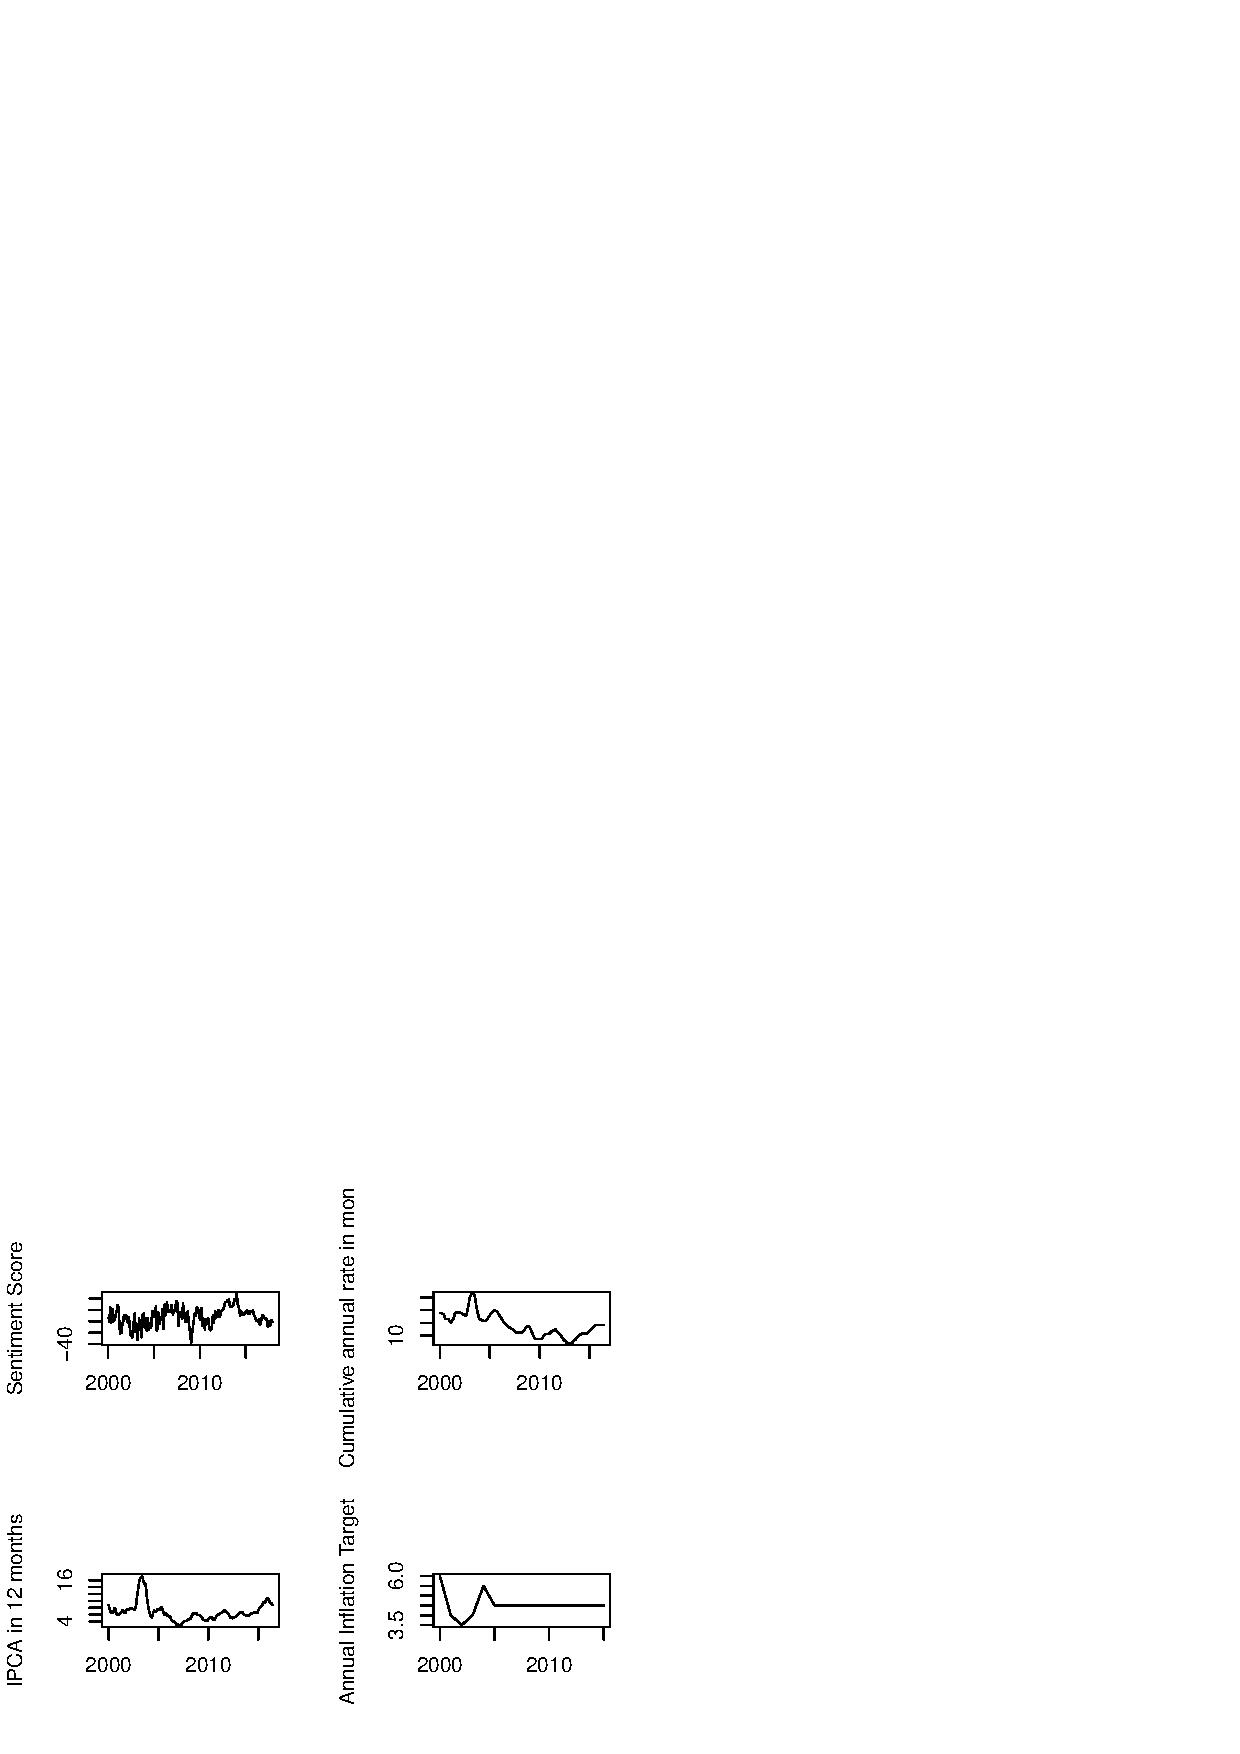
\includegraphics[width=3.5in]{comparative.png}
  \end{figure}
\end{frame}

%%%
% CONCLUSÕES
%%%

\subsection{Conclusão}

\begin{frame}\frametitle{Conclusões}
  \begin{itemize}
    \item Expomos a aplicação de \emph{Text Mining} nas atas das reuniões do Copom que são divulgadas no site do BCB;
    \item Utilizando técnicas de \emph{Web Scraping} e \emph{Text Mining} mostramos o índice de sentimento está relacionado com séries temporais importantes para a autoridade monetária (IPCA, Selic);
    \item Tal resultado fortalece a importância do uso das técnicas apresentadas em pesquisa ecocômicas aplicadas;
    \item No que tange aos resultados empíricos, testes comumente utilizados em séries temporais como Causalidade de Granger podem contribuir para a robustez dos resultados assim como o uso da série temporal do índice de sentimento em modelos VAR, SVAR, VEC ou SVEC;
    \item Além disso, trabalhos futuros podem usar a mesma base de dados em busca de predizer as decisões do BCB por meio de técnicas de \emph{Machine Learning};
    \item Por fim, a mesma metodologia de acesso aos dados pode ser empregada em outros documentos divulgados pela autoridade monetária (relatórios de inflação, comunicados, carta aberta)
  \end{itemize}
\end{frame}

\end{document}



